\chapter{初态的 Wigner 抽样}
\label{ch:initial-sampling}

\begin{learningobjectives}
完成本章后，读者应能：
\begin{enumerate}
  \item 精确抽样相干态、热态和一般正高斯 Wigner 分布；
  \item 用 Bogoliubov 模式构造量子与热涨落，并检查其辛归一化；
  \item 为参数淬火生成包含压缩关联的初态协方差；
  \item 识别定粒子数约束、零模和非正 Wigner 函数带来的限制。
\end{enumerate}
\end{learningobjectives}

\section{先定义量子态，再选择随机数}

初态抽样不是给平均场“随手加一点噪声”。每一条轨迹必须来自一个明确量子态的 Wigner 函数，或者来自一个声明过矩匹配范围的近似分布。推荐按以下顺序工作：
\begin{enumerate}
  \item 指定密度算符或高斯态的一、二阶矩；
  \item 选定第10章的有限模式基与截止；
  \item 把目标矩转换为对称排序协方差；
  \item 生成随机样本，并在进入动力学前回测这些矩。
\end{enumerate}
直接从随机数分布出发，常会把每模半量子、热粒子或真实耗尽重复加入。
高斯协方差和辛变换的通用背景见\cite{Weedbrook2012}；对凝聚体零模
与数守恒 BdG 的更严格处理可参见\cite{Castin1998}。

\section{相干态与真空}

若第 $n$ 个模式处于相干态 $|\bar\alpha_n\rangle$，其 Wigner 抽样为
\begin{equation}
  \alpha_n=\bar\alpha_n+\frac{\xi_{1n}+\ii\xi_{2n}}{2},
  \qquad
  \xi_{1n},\xi_{2n}\sim\mathcal N(0,1).
  \label{eq:coherent-mode-sampling}
\end{equation}
于是
\begin{equation}
  \ensavg{\alpha_n}=\bar\alpha_n,
  \quad
  \ensavg{|\alpha_n-\bar\alpha_n|^2}=\frac12,
  \quad
  \ensavg{(\alpha_n-\bar\alpha_n)^2}=0.
  \label{eq:coherent-mode-moments}
\end{equation}
真空是 $\bar\alpha_n=0$ 的特例。若经典平均场展开为
$\psi_0(x)=\sum_n\phi_n(x)\bar\alpha_n$，则场样本为
\begin{equation}
  \psi(x)=\psi_0(x)
  +\frac12\sum_{n\in\mathcal C}\phi_n(x)
  (\xi_{1n}+\ii\xi_{2n}).
  \label{eq:coherent-field-sampling}
\end{equation}
在实空间正交格点基中，它退化为式\eqref{eq:grid-vacuum-sampling}除以 $\sqrt{\Delta x}$。

一个相干态的正规排序平均粒子数是 $|\bar\alpha_n|^2$，但单条轨迹的 $|\alpha_n|^2-1/2$ 可以为负。Wigner 轨迹不是单次实验中可直接观测的微观态；只有按正确估计器取系综平均才有量子意义。

\section{热高斯模式}

频率为 $\omega_n$、化学势已经包含在准粒子能量定义中的独立热模式具有
\begin{equation}
  \bar n_n=\frac{1}{\exp(\beta\hbar\omega_n)-1}.
\end{equation}
其 Wigner 函数是正高斯分布，可精确抽样为
\begin{equation}
  \alpha_n=\sqrt{\frac{\bar n_n+1/2}{2}}
  (\xi_{1n}+\ii\xi_{2n}),
  \label{eq:thermal-mode-sampling}
\end{equation}
从而
\begin{equation}
  \ensavg{|\alpha_n|^2}=\bar n_n+\frac12.
  \label{eq:thermal-wigner-moment}
\end{equation}
高温极限下 $\bar n_n\simeq k_BT/(\hbar\omega_n)$，但在低占据模式中用这一经典近似替换 Bose--Einstein 分布会高估热尾部。半量子 $1/2$ 也不能再额外叠加到式\eqref{eq:thermal-mode-sampling}上。

\section{一般高斯协方差的抽样}

对 $M$ 个模式引入实正交变量
\begin{equation}
  \bm R=(Q_1,P_1,\ldots,Q_M,P_M)^T,
  \qquad
  \alpha_n=(Q_n+\ii P_n)/\sqrt2.
\end{equation}
高斯态由均值 $\bar{\bm R}$ 和对称排序协方差
\begin{equation}
  V_{jk}=\frac12\qavg{
  \Delta\hat R_j\Delta\hat R_k+
  \Delta\hat R_k\Delta\hat R_j}
  \label{eq:gaussian-covariance-definition}
\end{equation}
决定。若 $V=LL^T$ 是 Cholesky 分解，则
\begin{equation}
  \bm R=\bar{\bm R}+L\bm\xi,
  \qquad
  \bm\xi\sim\mathcal N(\bm0,\identity_{2M}).
  \label{eq:initial-gaussian-cholesky-sampling}
\end{equation}
可直接生成样本。数值上必须先检查 $V$ 对称且正定；物理上还须满足不确定关系
\begin{equation}
  V+\frac{\ii}{2}\Omega\succeq0,
  \label{eq:gaussian-uncertainty}
\end{equation}
其中 $\Omega=\bigoplus_n\begin{pmatrix}0&1\\-1&0\end{pmatrix}$。一个正定矩阵未必是合法量子协方差。

对于强压缩态，$V$ 的特征值跨度可能很大。直接 Cholesky 分解前宜先对称化 $V\leftarrow(V+V^T)/2$，并用辛本征值而非只看普通特征值检查不确定关系。由舍入产生的微小负特征值可以在明确容差内诊断；不能无记录地裁剪一个实质上非物理的协方差。

\section{Bogoliubov 真空与有限温初态}

设 $\psi_0(x)$ 是定态 Gross--Pitaevskii 解。在破缺 $U(1)$ 对称的 Bogoliubov 表示中，涨落算符写成
\begin{equation}
  \delta\hpsi(x)=
  \sum_{\nu\in\mathcal B}
  \left[u_\nu(x)\hb_\nu-v_\nu^*(x)\hbd_\nu\right].
  \label{eq:bogoliubov-expansion}
\end{equation}
正能模满足辛归一化
\begin{equation}
  \int\dd x\,
  \left[u_\nu^*(x)u_\mu(x)-v_\nu^*(x)v_\mu(x)\right]
  =\delta_{\nu\mu}.
  \label{eq:bogoliubov-normalization}
\end{equation}
相应场样本为
\begin{equation}
  \psi(x)=\psi_0(x)+
  \sum_{\nu\in\mathcal B}
  \left[u_\nu(x)b_\nu-v_\nu^*(x)b_\nu^*\right],
  \label{eq:bogoliubov-field-sampling}
\end{equation}
其中
\begin{equation}
  b_\nu=\sqrt{\frac{\bar n_\nu+1/2}{2}}
  (\xi_{1\nu}+\ii\xi_{2\nu}).
  \label{eq:bogoliubov-mode-sampling}
\end{equation}
取 $\bar n_\nu=0$ 得 Bogoliubov 真空，有限温则用准粒子能量 $\epsilon_\nu$ 计算
$\bar n_\nu=[\exp(\beta\epsilon_\nu)-1]^{-1}$。

式\eqref{eq:bogoliubov-field-sampling}中的 $v$ 项意味着即使准粒子真空也可以含有真实原子耗尽：
\begin{equation}
  N_{\rm dep}^{(0)}=\sum_\nu\int\dd x\,|v_\nu(x)|^2.
  \label{eq:quantum-depletion}
\end{equation}
这与每个数值模式的对称排序半量子不是同一对象。前者是 Bogoliubov 变换后正规排序原子数，后者是 Wigner 表示基线。

为与第4章一致，本书固定单模压缩约定
$c=\cosh r\,b-\sinh r\,b^*$。因此 $r>0$ 压缩
$Q=(c+c^*)/\sqrt2$，并给出
$\Var(Q)=\ee^{-2r}/2$、$\Var(P)=\ee^{2r}/2$ 以及
$\ensavg{c^2}=-\sinh(2r)/2$。若文献采用相反的加号，压缩轴和反常矩符号会
同时交换；这只是相位约定，但公式、代码和图必须成套一致。

\subsection{零模与完备性}

破缺连续对称性会产生零能或近零能模，其范数和热占据公式可能奇异。不能把 $\epsilon_\nu=0$ 直接代入 Bose 因子。常见处理包括固定整体相位、采用数守恒 Bogoliubov 理论，或把集体坐标单独量子化。无论采用哪种方式，都应检查保留的 $(u,v)$ 模是否满足辛正交与所需完备关系，并报告排除了哪些零模。

\section{淬火与压缩关联}

若初态是淬火前哈密顿量 $H_i$ 的热平衡态，而 $t=0$ 后按 $H_f$ 演化，最安全的流程是在 $H_i$ 的准粒子基中抽样，再转换到实际传播场。设前后准粒子满足
\begin{equation}
  c_\mu=\sum_\nu\left(A_{\mu\nu}b_\nu+B_{\mu\nu}b_\nu^*\right).
  \label{eq:quench-bogoliubov-map}
\end{equation}
即使初态中 $\ensavg{b_\nu b_\mu}=0$，淬火后变量通常具有
$\ensavg{c_\mu c_\lambda}\neq0$ 的反常协方差。这正是成对激发和压缩的相空间信号。

在两套数值 BdG 模之间转换时，矩阵 $A,B$ 必须保持玻色对易关系，例如
\begin{equation}
  AA^\dagger-BB^\dagger=\identity,
  \qquad
  AB^T-BA^T=0.
  \label{eq:bogoliubov-map-constraints}
\end{equation}
这些等式是比“图看起来像压缩”更敏感的实现测试。

\section{定粒子数不是简单归一化}

相干态平均场的总粒子数本来就有 Poisson 涨落。逐轨迹把所有场强制归一到同一个 $N$，会改变径向分布与相位--数关联，因此不再抽样原相干态。另一方面，Fock 态的 Wigner 函数具有振荡和负值，不能由普通正概率精确抽样。

常用近似是给凝聚模取固定半径 $|\alpha_0|\simeq\sqrt{N_0+1/2}$ 和随机整体相位，或先抽样正交涨落再调节凝聚占据以满足总数约束。这些方案可以匹配某些低阶矩，却不是 Fock 态 Wigner 函数的精确正抽样。使用时应说明：匹配哪些矩、误差按什么大参数受控、整体相位是否与目标观测量相关。

\begin{warningbox}
“每条轨迹粒子数相同”是一项状态建模选择，不是自动提高精度的数值技巧。任何重缩放都会改变抽样分布；必须在重缩放后重新检查目标一、二阶矩。
\end{warningbox}

\section{抽样验收测试}

在传播前至少完成以下检查：
\begin{enumerate}
  \item 每个独立模式的均值、$\ensavg{|\Delta\alpha|^2}$ 和反常矩 $\ensavg{(\Delta\alpha)^2}$；
  \item 场的一体密度矩阵与目标协方差；
  \item 正规排序总粒子数、能量和耗尽；
  \item BdG 模的辛范数、正交性和正负能配对；
  \item 样本数加倍后，偏差是否按统计误差缩小；
  \item 更换随机种子后，结论是否落在预先给定的置信区间内。
\end{enumerate}
本章配套程序从真空圆高斯通过单模 Bogoliubov 变换生成压缩真空，并把样本协方差与解析值比较，结果见\cref{fig:squeezed-sampling}。
\begin{figure}[htbp]
  \centering
  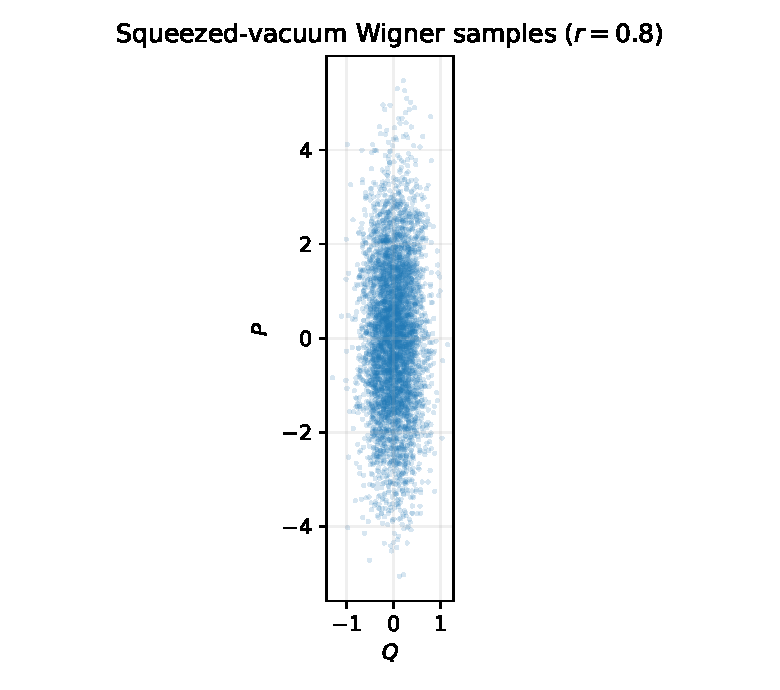
\includegraphics[width=0.72\textwidth]{figures/ch11/squeezed_wigner_sampling.pdf}
  \caption[压缩真空的 Wigner 抽样基准]{压缩参数 $r=0.8$ 时的单模压缩真空 Wigner 抽样。散点显示 $100000$ 个实际随机样本中的子集，椭圆给出解析高斯协方差；全样本协方差与反常矩的最大偏差分别为 $0.82$ 与 $0.84$ 个标准误以内。该图只验证单模高斯变换和抽样，不验证非高斯初态或后续相互作用动力学。}
  \label{fig:squeezed-sampling}
\end{figure}
图中的点是实际随机样本，不是示意性手绘；运行参数与数值误差保存在
\path{data/ch11/squeezed_sampling_metrics.json}。

\begin{chaptercheck}
把相互作用和传播时间都设为零，只运行初态生成器。若抽样的一、二阶矩不能在预期的 $N_s^{-1/2}$ 误差内复现输入协方差，就不应进入淬火模拟。初态偏差不会被更高阶积分器修复。
\end{chaptercheck}

\section*{本章小结}

相干态、热态和正高斯态可以直接由其实协方差精确抽样；Bogoliubov 初态还要求模式的辛归一化、零模处理与原子/准粒子基之间的一致转换。参数淬火会把普通协方差变成包含反常矩的压缩关联。固定粒子数和强非经典态则需要明确的近似或替代表示，不能靠轨迹重归一化假装精确。

\begin{exercises}
  \item 由式\eqref{eq:thermal-mode-sampling}计算 $Q,P$ 两个无量纲正交分量的方差。
  \item 证明式\eqref{eq:bogoliubov-map-constraints}保证变换后的 $c_\mu$ 仍满足玻色对易关系。
  \item 对单模压缩参数 $r$，取 $c=\cosh r\,b-\sinh r\,b^*$，求两个正交分量的方差与反常矩，并验证 $r>0$ 压缩 $Q$ 轴。
  \item 说明为什么逐轨迹归一化会在相干态中引入模式间关联。
  \item 为一个含 Goldstone 零模的 BdG 数值谱设计筛选、归一化和完备性检查。
\end{exercises}
